\documentclass{article}
\usepackage[margin=2cm]{geometry}
\usepackage{graphicx}
\usepackage{hyperref}
\hypersetup{
	colorlinks=true,
	linkcolor=blue,
	filecolor=magenta,      
	urlcolor=cyan,
}

\title{{\Huge Net Computing} \\[.5cm] {\Large Nodes Measurement System}}
\author{
\begin{tabular}{r l}
	Martijn Luinstra & s\,2199289 \\
	Emilio Oldenziel & s\,2509679 \\
	Yannick Stoffers & s\,2372061
\end{tabular}
}

\begin{document}
\maketitle

\section{Introduction}
	% What our application does %
	% Written by Emilio.
	% Yannick spellchecked and completed.
	We have created a nodes measurement system, with which a user can monitor nodes 
	(or any other machine) in a network. To do this we created a multi-platform
	application existing of three parts, the first one is the server which is the
	part which is the core of our application, this server handles the setup of
	the nodes and clients, handles messages coming from either and does the 
	required administration. The second part is the node part, this piece of 
	software can be run on any machine and connects to the central server, then it
	proceeds to measure the machines hardware and sends the measurements to the 
	server. The last part are the clients which can connect to the central 
	server with their browser to see a dashboard with the measurements from all 
	nodes. On this web interface the user has the ability to shut down the 
	network, or for illustrative purposes play the Wilhelm scream.
	

\newpage
\section{Architecture}
	% Overview of how the system is set-up %
	% Written by Emilio.
	The system consists of a central server, nodes that are measured and clients
	that are connected to the central server with their browser. The nodes send 
	their measurements to the central server using message queueing, the central
	server has a worker that handles the message queue and takes the measurement
	from the queue and than processes them. The worker saves the measurement in 
	a database for archiving purposes and sends the measurement directly to the 
	client's browser using the browser's websockets. More nodes that have to be
	measured can be added by using web services, the node asks the central 
	server if he can be monitored, if that is possible, the central server gives
	setup data to the node like what its id is and where he has to queue his 
	measurements.
	
	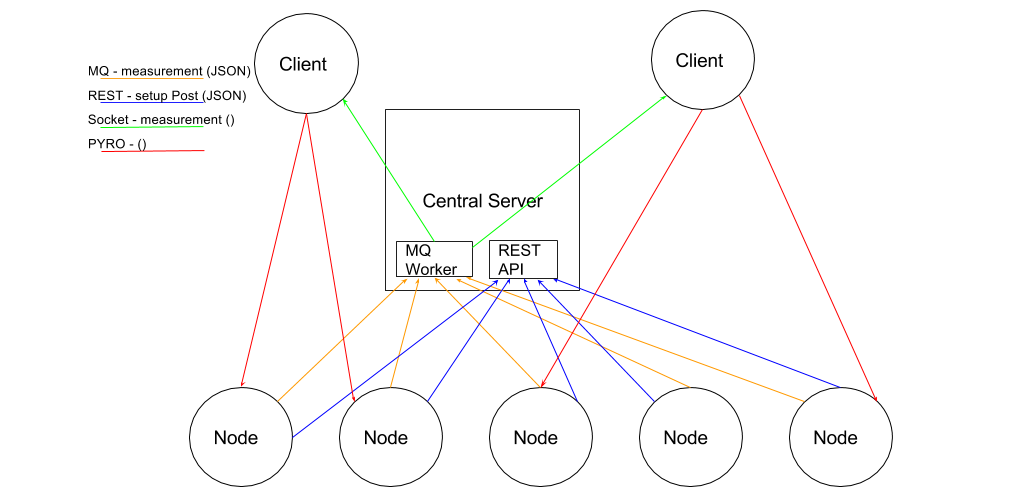
\includegraphics[scale=0.45]{architecture.png}

\section{Design choices}
	%explain why we used one central server with workers instead of p2p
	We chose to have a central server so that we have one point that 
	does the `bookkeeping' of which nodes are monitored, but also to 
	make it simpler that nodes and client connect to the same point.
	
	%Why we chose python
	The language that we used for this project is Python, we chose that 
	because we all have a lot more experience with Python than with Java. For 
	projects like this where we have to show that we understand the concepts 
	and techniques, Python is nicer because we don't have to deal with the
	generics of Java and can concentrate more on the main concepts. Speed is 
	not an issue in this system because Python is fast enough to handle all 
	the operations without human noticeable latency.
	
	% explain why we used JSON %
	We used JSON as datatype for our communication, mainly because it is very 
	simple to use in python. There is a standard JSON library in python 
	that can create a JSON object from a dictionary (python version of a 
	HashMap) and vice versa.
	In this way we could serialize our data in a simple way and then send it.
	JSON is nowadays the most used data-type for sending objects over the 
	internet because of its simplicity and human-readability. %vague remark%
	
\section{Application Flow}
	First the central server and its workers are started. A node can ask the 
	server if he can be observed and gives his name and ip-address, the server 
	responds with No or gives the setup data. Once the node received the setup 
	data the node will start a worker thread that does measurements from the 
	hardware and queues this to the message queue of the central worker, the 
	node will continue doing this every second until the thread is stopped. 

	The central server's message queue worker will save the measurement and 
	send it directly to all connected browsers. If a node has a major difference
	in some metric (e.g. the CPU temperature will increase very rapidly) this 
	will be seen on the dashboard on the browser. 

	In the browser, when a user presses a button, a server side python method is 
	invoked. This method searches for the pyro name server. This name server 
	keeps a record of all the connected objects on which methods can be invoked.
	The method continues by invoking a single method on all the found objects.
	These objects will then either attempt to shut down the system or play a
	lovely sound sample. This final step is thus executed on the connected nodes.

	Below the class diagram is displayed.
	
	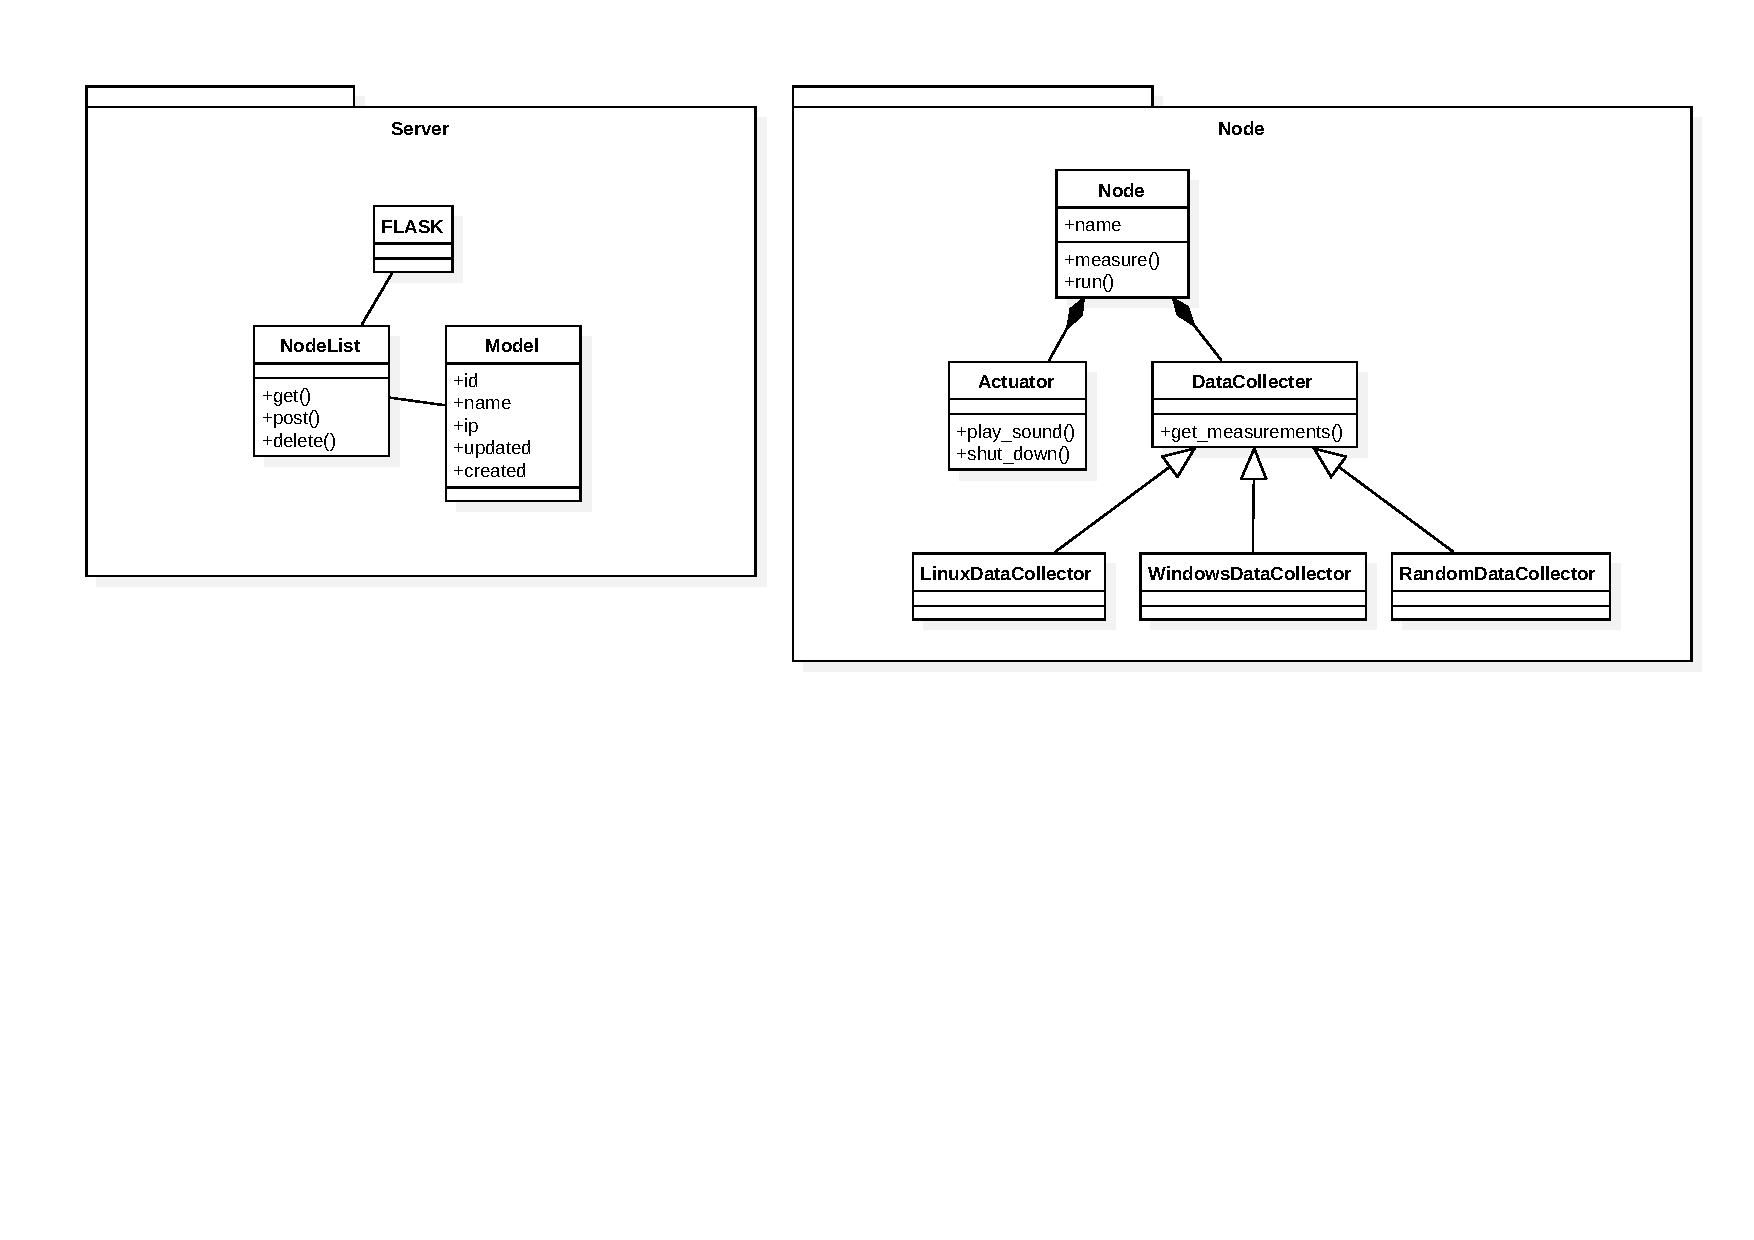
\includegraphics[width=\textwidth, trim={60 250 0 0}]{classdiagram.pdf}

\section{Techniques}
	%Flask (API, Server, Models, sockets), RabbitMQ(Pika), PYRO
	We made use of multiple frameworks for this project. For the central server
	we used \href{http://flask.pocoo.org/}{Flask} with the 
	\href{https://flask-restful.readthedocs.io/en/0.3.5/}{Flask-Restful} API to
	do the initial setup of a node, this API uses REST to handle requests. As
	server for the API we used the development server of Flask, this is a 
	lightweight server that has everything to demonstrate the application. To 
	store the measurements 
	\href{http://flask-sqlalchemy.pocoo.org/2.1/}{Flask SQL-alchemy} is used 
	with an SQLite database for simple storage of data from the demo.
	
	For Message queueing \href{https://www.rabbitmq.com}{RabbitMQ} is used, to 
	use RabbitMQ with python we used \href{https://github.com/pika/pika}{pika}, 
	which is a Python interface for RabbitMQ. 

	The front end connects to the central server using websockets. These 
	websockets simply send all data from the server to the frontend.

	Finally, in order to invoke a method on a node itself we created a simple 
	python class that is exposed to the name pyro name server. In other words, 
	we used the \href{https://pythonhosted.org/Pyro4/}{Pyro4} library.

\section{Difficulties}
	% RabbitMQ? %
	Some difficulties we experienced were mainly setup related. Getting rabbitmq
	to allow for external connections by removing loopback restrictions of the 
	default user, and realising the pyro name server is hosted on localhost by 
	default. Furthermore finding the proper libraries for everything that we 
	wanted to do wasn't a breeze at all. Although many were relatively easy to 
	find, we still couldn't find a single Python library that allows for easy 
	access to hardware sensors in MacOS. Developing the product and setting up 
	the idea was a rather straightforward process, and overall we are quite 
	satisfied.

\section{Conclusion}
	In this project we wanted to build something that was simple but had all
	mandatory components in it. For each part we picked the technique that 
	was the most logical, mostly based on frequency of use and speed, but also in
	such a way that all parts were implemented with a different one. Using 
	Python we had a lot of libraries and frameworks to choose from, we used 
	the ones that we though that got the job done in the simplest way or we 
	already had experience with, such as Flask. Doing this it saved us a lot of 
	time because we already know and/or minimized the struggles that come with 
	such frameworks. 

\section{Evaluation}
	All in all we think that we have learned a lot of things that are very 
	practical to have knowledge of. This can become very useful for later 
	projects that need a way of communication between machines. We now know 
	which techniques are most suitable for certain applications or architectures.
	% more bladibladi bla ...

\end{document}
